%%%%%%%%%%%%%%%%%%%%%%%%%%%%%%%%%%%%%%%%%%%%%%%%%%%%%%%%%%%%%%%%%%%%%%%%%%%%
% 26/05/2010
% edited by Bill Lampos
%
% Feel free to use (copy) the structure (latex formatting source code)
% but not the content of this document.
%
%%%%%%%%%%%%%%%%%%%%%%%%%%%%%%%%%%%%%%%%%%%%%%%%%%%%%%%%%%%%%%%%%%%%%%%%%%%%%
\documentclass[compress,red]{beamer}
\mode<presentation>


\usetheme{Warsaw}
% other themes: AnnArbor, Antibes, Bergen, Berkeley, Berlin, Boadilla, boxes, CambridgeUS, Copenhagen, Darmstadt, default, Dresden, Frankfurt, Goettingen,
% Hannover, Ilmenau, JuanLesPins, Luebeck, Madrid, Maloe, Marburg, Montpellier, PaloAlto, Pittsburg, Rochester, Singapore, Szeged, classic

%\usecolortheme{lily}
% color themes: albatross, beaver, beetle, crane, default, dolphin, dov, fly, lily, orchid, rose, seagull, seahorse, sidebartab, structure, whale, wolverine

%\usefonttheme{serif}
% font themes: default, professionalfonts, serif, structurebold, structureitalicserif, structuresmallcapsserif

% pdf is displayed in full screen mode automatically
%\hypersetup{pdfpagemode=FullScreen}

% define your own colours:
\definecolor{Red}{rgb}{1,0,0}
\definecolor{Blue}{rgb}{0,0,1}
\definecolor{Green}{rgb}{0,1,0}
\definecolor{magenta}{rgb}{1,0,.6}
\definecolor{lightblue}{rgb}{0,.5,1}
\definecolor{lightpurple}{rgb}{.6,.4,1}
\definecolor{gold}{rgb}{.6,.5,0}
\definecolor{orange}{rgb}{1,0.4,0}
\definecolor{hotpink}{rgb}{1,0,0.5}
\definecolor{newcolor2}{rgb}{.5,.3,.5}
\definecolor{newcolor}{rgb}{0,.3,1}
\definecolor{newcolor3}{rgb}{1,0,.35}
\definecolor{darkgreen1}{rgb}{0, .35, 0}
\definecolor{darkgreen}{rgb}{0, .6, 0}
\definecolor{darkred}{rgb}{.75,0,0}

\xdefinecolor{olive}{cmyk}{0.64,0,0.95,0.4}
\xdefinecolor{purpleish}{cmyk}{0.75,0.75,0,0}

% \usepackage{beamerinnertheme_______}
% inner themes include circles, default, inmargin, rectangles, rounded

%\usepackage{beamerouterthemesmoothbars}
% outer themes include default, infolines, miniframes, shadow, sidebar, smoothbars, smoothtree, split, tree

\useoutertheme[subsection=false]{smoothbars}

% to have the same footer on all slides
%\setbeamertemplate{footline}[text line]{xxx xxx xxx}
%\setbeamertemplate{footline}[text line]{} % or empty footer

% include packages
\usepackage{subfigure}
\usepackage{multicol}
\usepackage{amsmath}
\usepackage{epsfig}
\usepackage{graphicx}
\usepackage[all,knot]{xy}
\xyoption{arc}
\usepackage{url}
\usepackage{multimedia}
\usepackage{hyperref}
\usepackage{setspace}
\usepackage{hanging}
\usepackage{natbib}
\usepackage{bibentry}
\bibliographystyle{apalike}
\usepackage{chngcntr}
\counterwithin*{footnote}{page}
\newcommand\footcite[1]{\footnote{\bibentry{#1}}\label{\thepage:#1}}
\newcommand\secondcite[1]{\textsuperscript{\ref{\thepage:#1}}}
\usepackage{lmodern}    \usepackage[labelformat=empty,font=scriptsize,skip=0pt,justification=justified,singlelinecheck=false]{caption}

%remove the icon
\setbeamertemplate{bibliography item}{}

%remove line breaks
\setbeamertemplate{bibliography entry title}{}
\setbeamertemplate{bibliography entry location}{}
\setbeamertemplate{bibliography entry note}{}
\title{Proyecto final}
\subtitle{High quality photometric reconstruction using a depth camera}
\author{Daniel M\'endez, Camila Sanhueza}
\institute{\\ \vspace{.10cm}Profesor Ad\'in Ram\'irez}
\date{\scriptsize Visi\'on por computador, Universidad Diego Portales\\ \vspace{.10cm}Julio 15, 2015}

\begin{document}

\frame{
	\titlepage
}

\section[\'Indice]{}
\frame{\tableofcontents}

\section{Marco te\'orico}
\subsection{Fotometr\'ia est\'ereo}
\frame{\frametitle{Fotometr\'ia est\'ereo calibrada}

\begin{picture}(320,250)
\put(10,70){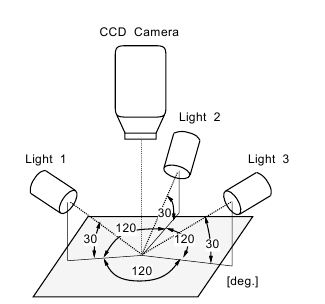
\includegraphics[width=0.5\textwidth]{photometric}}
\put(180,180){\begin{minipage}[t]{0.4\linewidth}
{Para realizar la fotometr\'ia estero se  calcular mediante:
\begin{equation}
I=n L,
\end{equation}
donde $I$ representa la intensidad de la imagen, $n$ las superficies normales de la imagen y $L$ las fuentes de iluminacion}
\end{minipage}}
\end{picture}

}

\frame{\frametitle{Superficie Lambertiana}
Las superficies Lambertianas los objetos a analizar tienen que ser mate.
\begin{figure}[p]
    \centering
    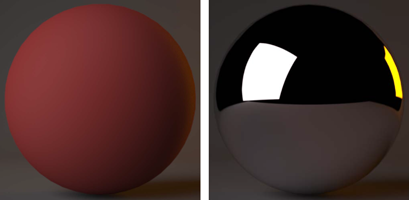
\includegraphics[width=0.5\textwidth]{lambertiana}
    \label{fig:awesome_image}
\end{figure}

}
\frame{\frametitle{Fotometr\'ia est\'ereo no calibrada}
La fotometr\'ia no calibrada se diferencia de la calibrada en:
\begin{itemize}
\item No se conoce la informaci\'on de la iluminaci\'on ni la intensidad. 

\item Para calcular las normales se utiliza la descomposici\'on de valores singulares.

\end{itemize}
}
\subsection{Teor\'ia documento de gu\'ia}
\frame{\frametitle{Fusi\'on de la estimaci\'on de la normal y la profundidad}
\begin{itemize}
\item Optimizaci\'on del mapa de profundidades:
\begin{equation}
\hat{Z}=E(\bar{Z})= E_{d}(\bar{Z})+\lambda_{n} E_{n}(\bar{Z})+\lambda_{s} E_{s}(\bar{Z})
\end{equation}
\item Penalizaci\'on de la profundidad

\begin{equation}
E_{d}(\bar{Z})= \sum_{p}w_{p}||\mu_{p}||^{2}(Z_{p}-\bar{Z_{p}})^{2}
\end{equation}

\end{itemize}

}

\frame{\frametitle{Fusi\'on de la estimaci\'on normal y la profundidad}
\begin{itemize}
\item Penalizaci\'on de la normal
\begin{equation}
E_n(\bar{Z})= \sum_{p}(N_{p}T_{x,p})^2+(N_{p}T_{y,p})^2
\end{equation}
\item Smoothness penalty
\begin{equation}
 E_{s}(\bar{Z})=\bigtriangledown^{2}(\bar{Z})
\end{equation}
\end{itemize}
}

\section{Dise\~no del c\'odigo}
\frame{\frametitle{Decisiones tomadas respecto a las dificultades presentadas}
Las decisiones fueron:
\begin{itemize}
\item Realizar una fotometr\'ia estero no calibrada.
\item Cambiar la iluminaci\'on infrarrojo, de una ampolleta infrarroja a una ampolleta hal\'ogena con filtro dicroico.
\item La cantidad de iluminaciones necesarias para la utilizaci\'on del c\'odigo.
\item Encontrar objetos con superficies Lambertianas.
\end{itemize}

\begin{columns}[t]
\column{.5\textwidth}
\centering
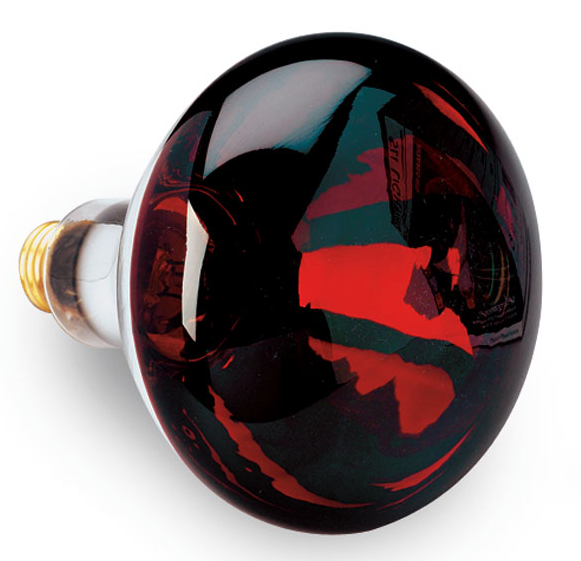
\includegraphics[width=0.5\textwidth]{ampolleta1}
\column{.5\textwidth}
\centering
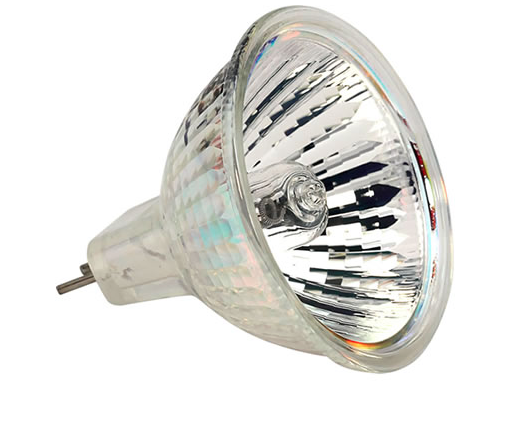
\includegraphics[width=0.6\textwidth]{ampolleta2}

\end{columns}

}

\section{Implementaci\'on del c\'odigo}
\subsection{Herramientas utilizadas}
\frame{\frametitle{Herramientas utilizadas}
Las herramientas utilizadas fueron:
\begin{itemize}
\item Openframeworks (ofxKinect)
\item OpenCv
\item Kinect
\item Ampolleta hal\'ogena con filtro dicroico
\end{itemize}

}
\subsection{Reutilizaci\'on de c\'odigo}
\frame{\frametitle{Reutilizaci\'on de c\'odigo}
Para poder realizar una fotometr\'ia est\'ereo no calibrada se utiliz\'o, un c\'odigo base, el creador es Kai Wolf.

}

\section{Experimentos}
\subsection{Set up prueba}
\frame{\frametitle{Set up prueba}
\begin{columns}[t]
\column{.5\textwidth}
\centering
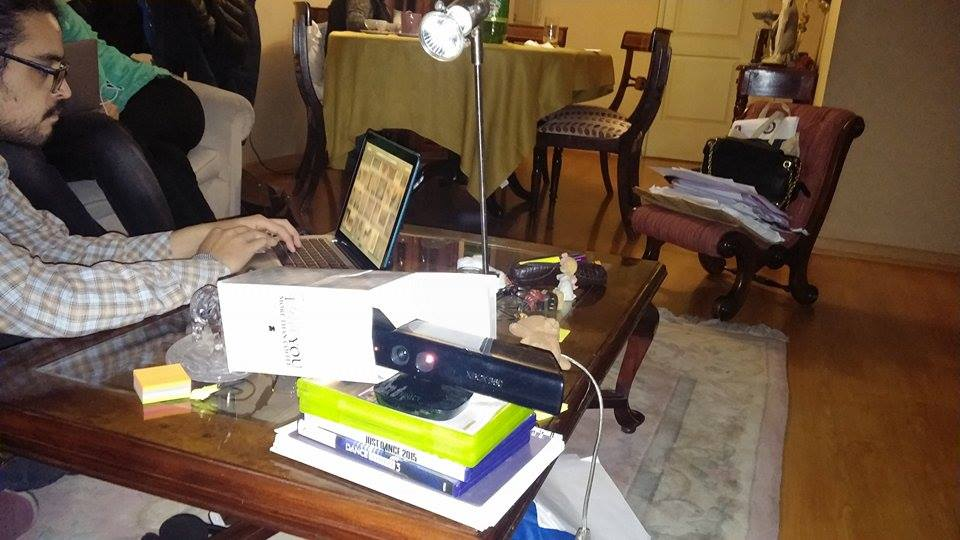
\includegraphics[width=1\textwidth]{setup1}\\
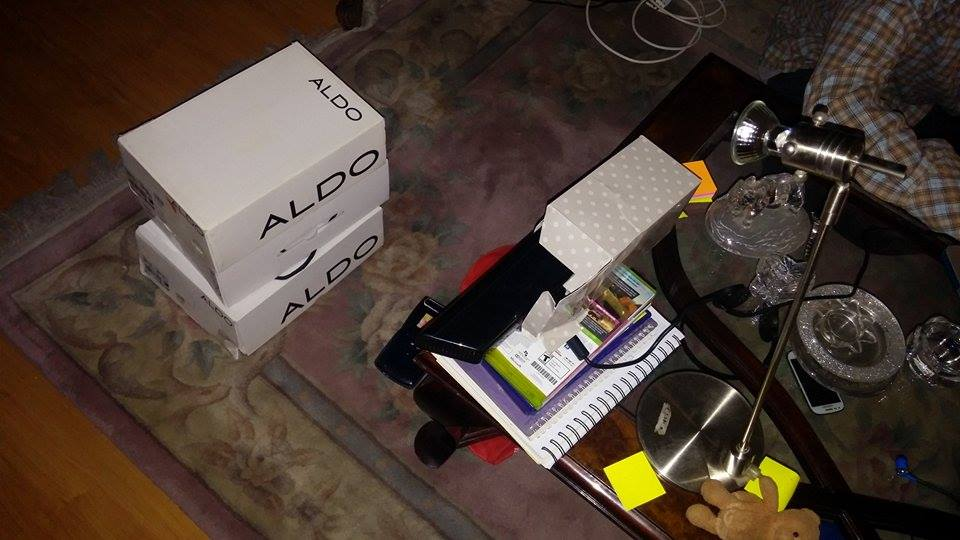
\includegraphics[width=1\textwidth]{setup2}

\end{columns}

}

\subsection{Resultados}
\frame{\frametitle{Set de im\'agenes necesarias para la reconstrucci\'on}
\begin{columns}[t]
\column{.5\textwidth}
\centering
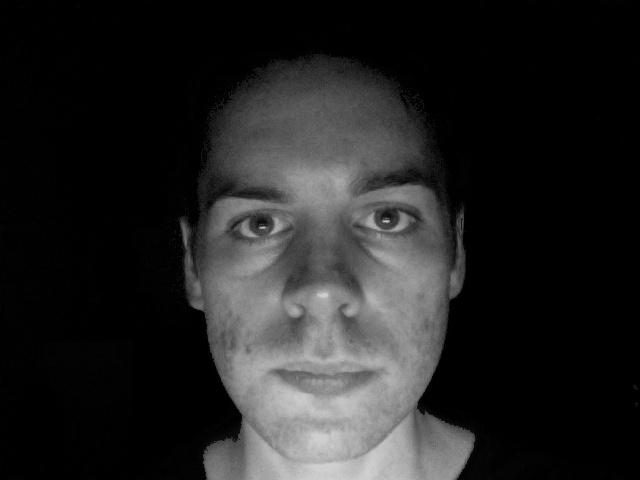
\includegraphics[width=0.8\textwidth]{0}\\
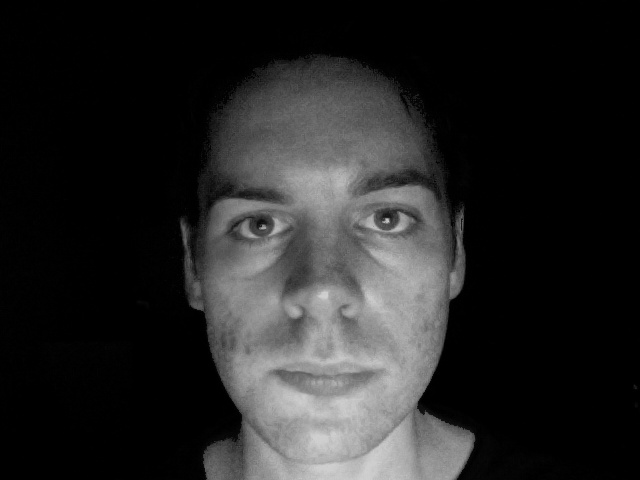
\includegraphics[width=0.8\textwidth]{1}
\column{.5\textwidth}
\centering
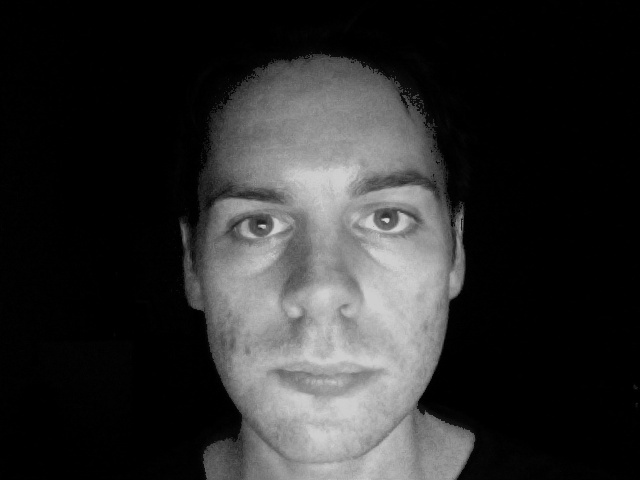
\includegraphics[width=0.8\textwidth]{2}\\
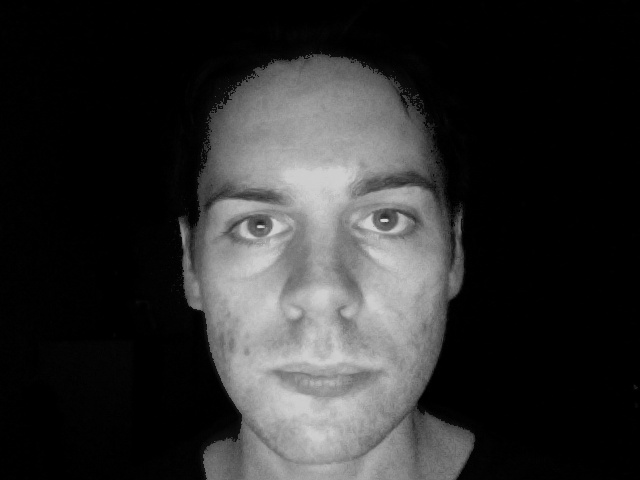
\includegraphics[width=0.8\textwidth]{3}
\end{columns}
}


\frame{\frametitle{Mascara de la imagen}


\includegraphics[width=0.9\textwidth]{Mascara1}

}
\frame{\frametitle{Mapa de normales}


\includegraphics[width=0.9\textwidth]{Normal1}


}

\frame{\frametitle{Mapa de profundidades estimado}

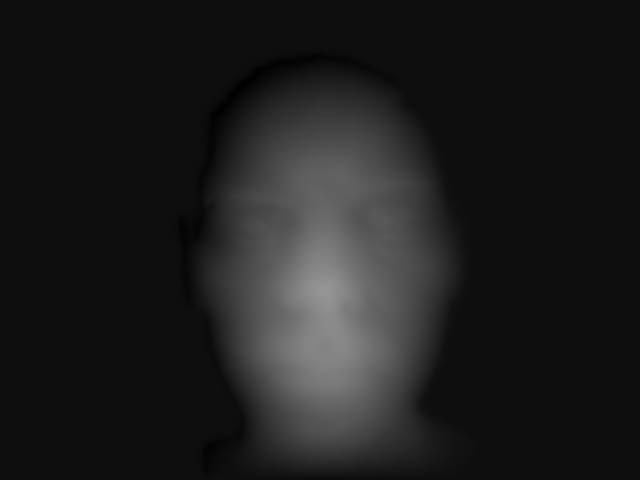
\includegraphics[width=0.9\textwidth]{Profundidad}


}

\frame{\frametitle{Reconstrucci\'on 3D }

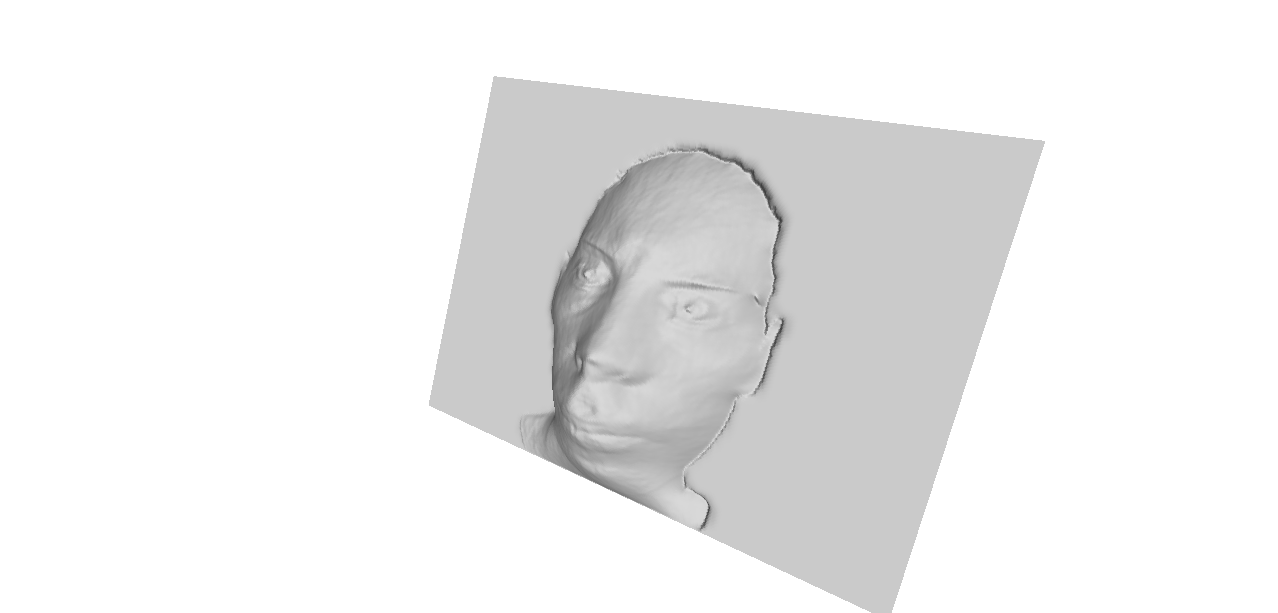
\includegraphics[width=1\textwidth]{nuestrowolf00}


}

\frame{\frametitle{Set de im\'agenes necesarias para la reconstrucci\'on}
\begin{columns}[t]
\column{.5\textwidth}
\centering
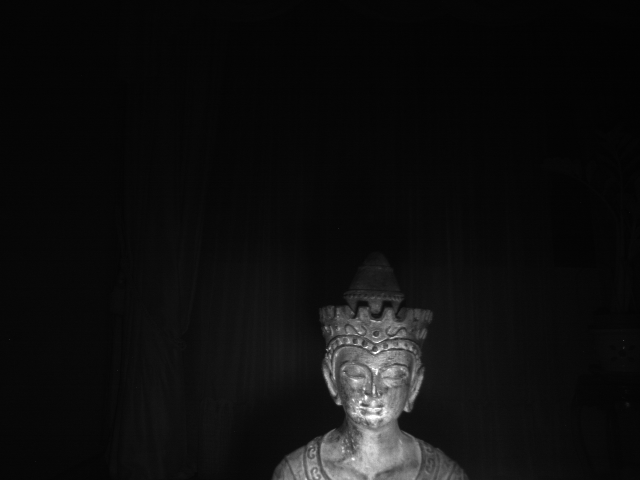
\includegraphics[width=0.8\textwidth]{02}\\
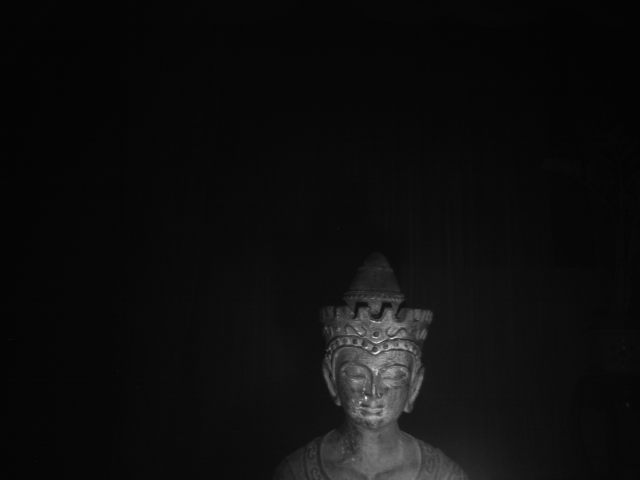
\includegraphics[width=0.8\textwidth]{12}
\column{.5\textwidth}
\centering
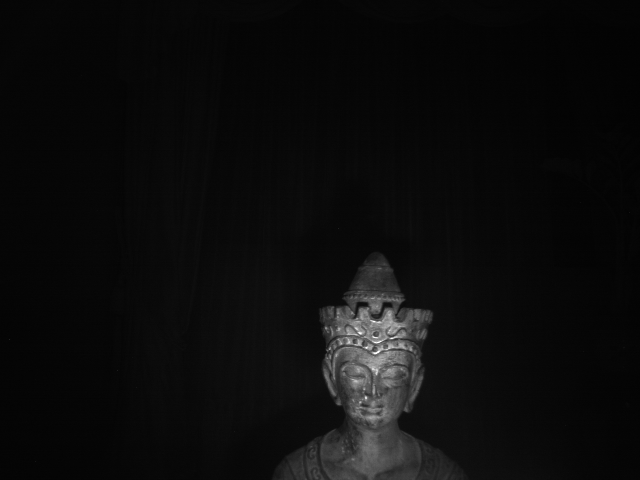
\includegraphics[width=0.8\textwidth]{22}\\
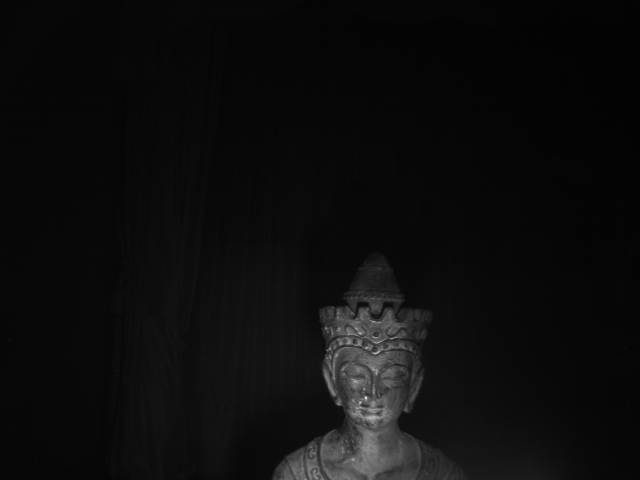
\includegraphics[width=0.8\textwidth]{32}
\end{columns}
}


\frame{\frametitle{Mascara de la imagen}

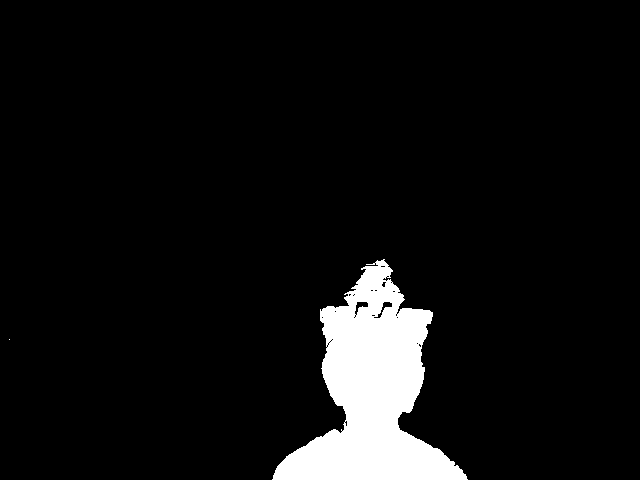
\includegraphics[width=0.9\textwidth]{Mascaramona}

}
\frame{\frametitle{Mapa de normales}

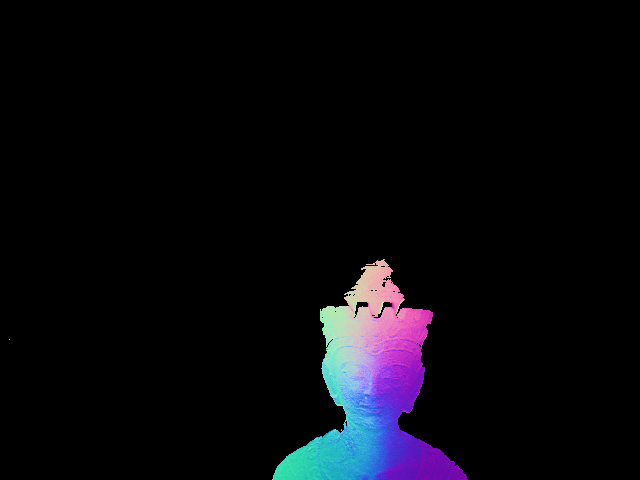
\includegraphics[width=0.9\textwidth]{Normalmona}


}

\frame{\frametitle{Mapa de profundidades estimado}

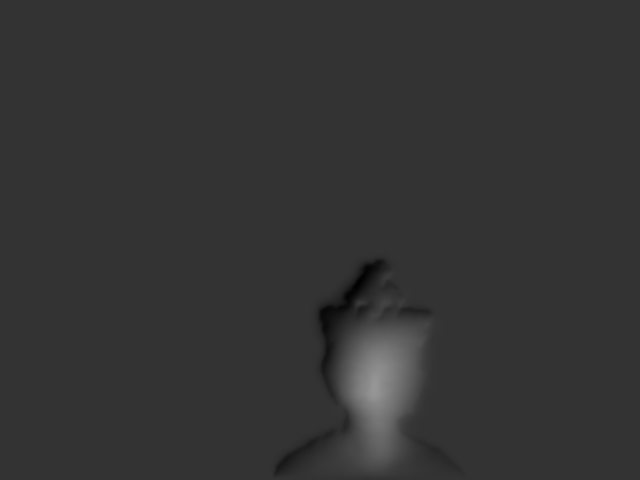
\includegraphics[width=0.9\textwidth]{Profundidadmona}


}

\frame{\frametitle{Reconstrucci\'on 3D }

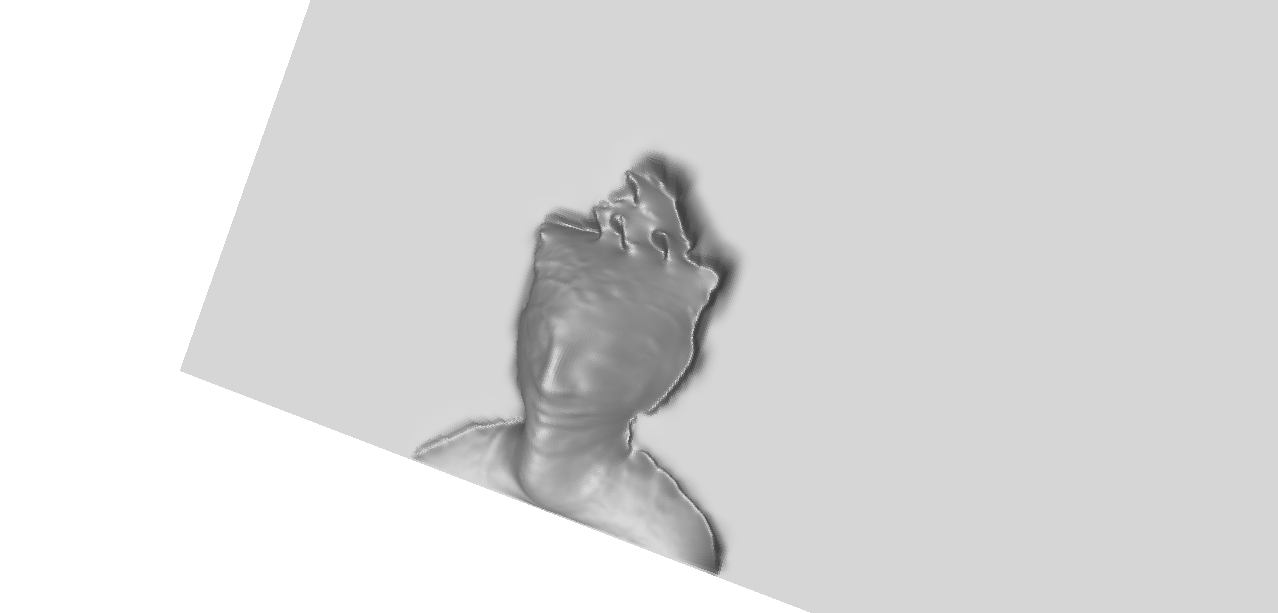
\includegraphics[width=1\textwidth]{3dmona01}


}

\frame{\frametitle{Set de im\'agenes necesarias para la reconstrucci\'on}
\begin{columns}[t]
\column{.5\textwidth}
\centering
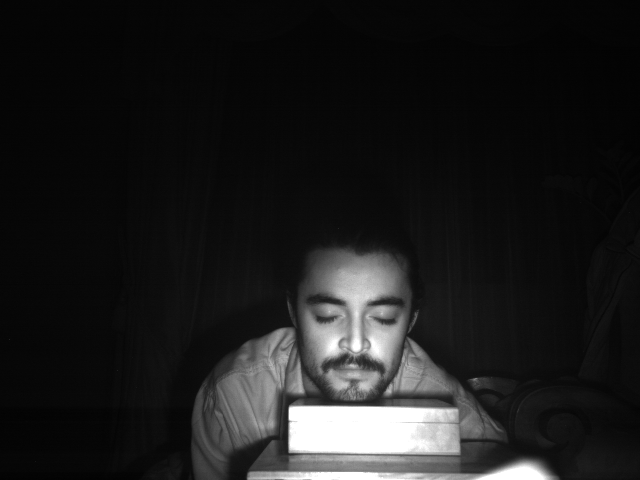
\includegraphics[width=0.8\textwidth]{03}\\
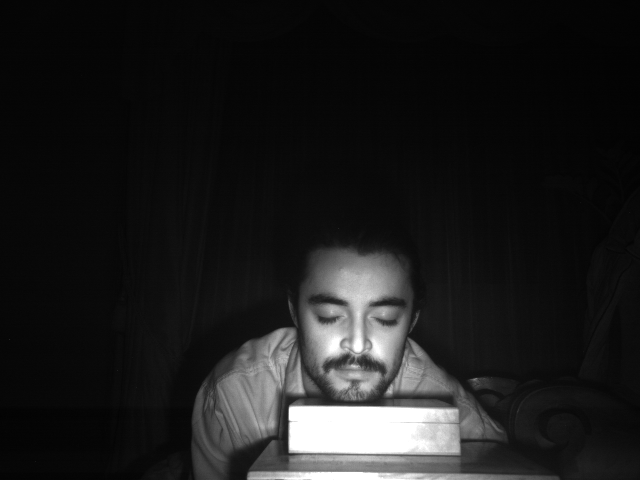
\includegraphics[width=0.8\textwidth]{13}
\column{.5\textwidth}
\centering
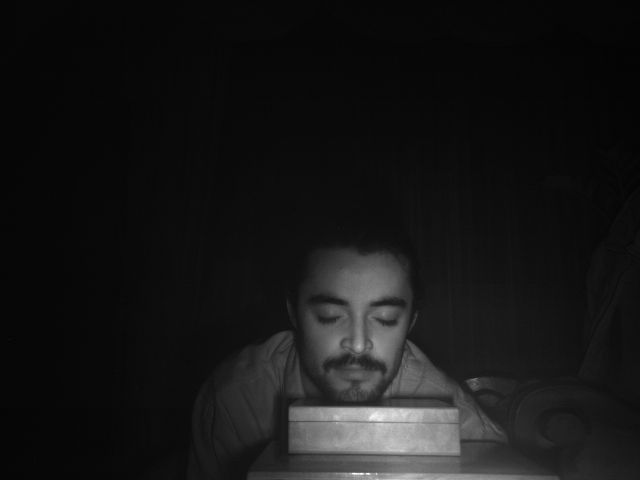
\includegraphics[width=0.8\textwidth]{23}\\
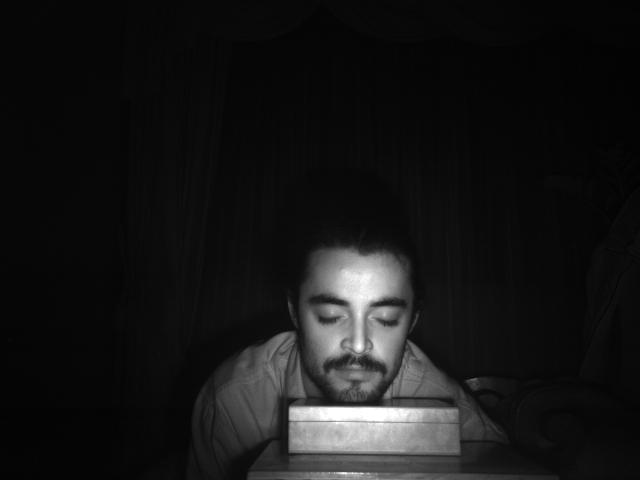
\includegraphics[width=0.8\textwidth]{33}
\end{columns}
}


\frame{\frametitle{Mascara de la imagen}

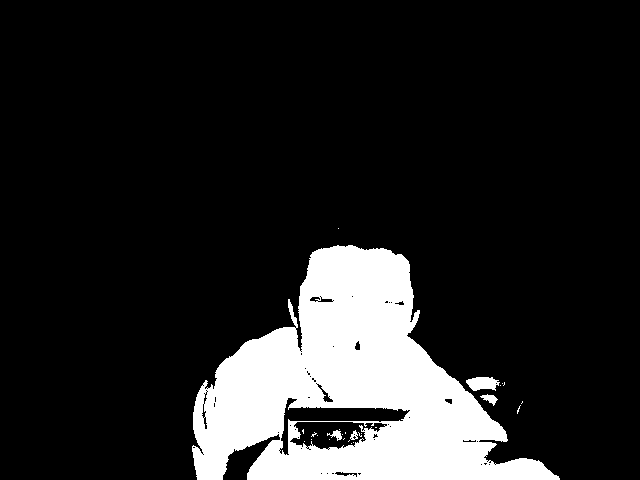
\includegraphics[width=0.9\textwidth]{Mascaracrepu}

}
\frame{\frametitle{Mapa de normales}

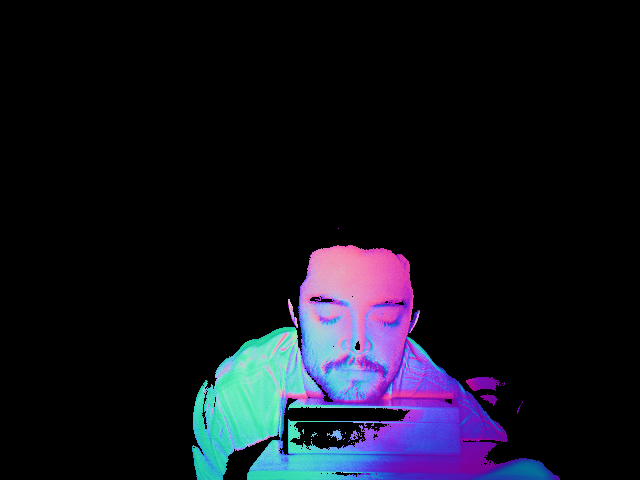
\includegraphics[width=0.9\textwidth]{Normalcrepu}


}

\frame{\frametitle{Mapa de profundidades estimado}

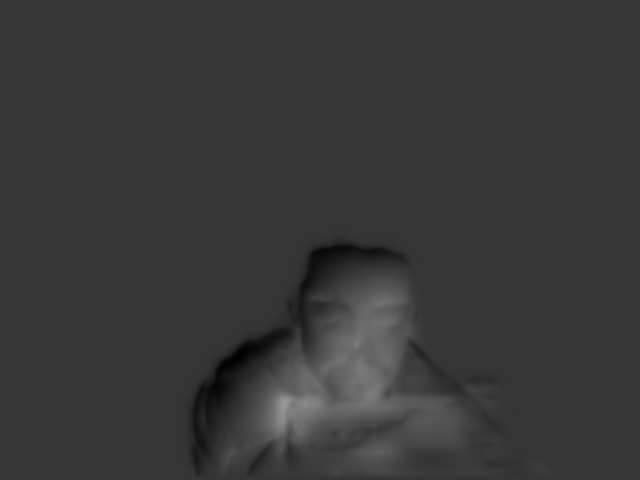
\includegraphics[width=0.9\textwidth]{Profundidadcrepu}


}

\frame{\frametitle{Reconstrucci\'on 3D }

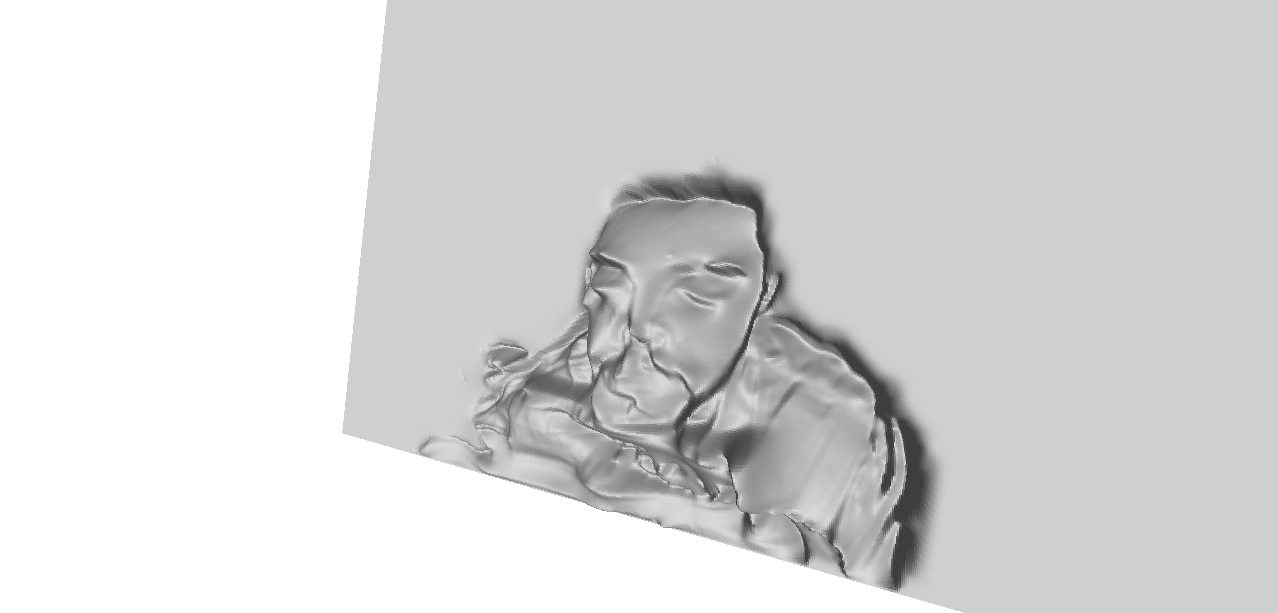
\includegraphics[width=1\textwidth]{3dcrepu00}


}

\section{Problemas}
\frame{\frametitle{Problemas al momento de el desarrollo}

Los principales problemas que se presentaron en el transcurso del proyecto final, fueron:
\begin{itemize}
\item La dificultad de poder hacer funcionar la Kinect.
\item La dificultad de comprender el procedimiento realizado por el texto gu\'ia (Haque, High Quality Photometric Reconstruction using a Depth Camera).
\item No saber como implementar ideas al momento de codificar. 
\end{itemize}
}

\section{Conclusiones}
\frame{\frametitle{Conclusiones}
\centering
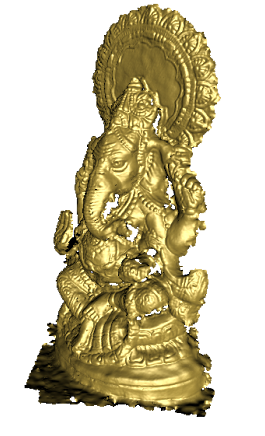
\includegraphics[width=0.45\textwidth]{conclu}
}


\end{document} 